\chapter{Performance evaluation}
\label{sec:perfeval}

The goals of the performance evaluation chapter is to validate the fact that the business application implemented with the generic stream processing library correctly react to an increasing event push rate on the Journal. From an initial push rate to a threshold, we expect the end-to-end latency\footnote{The duration between the moment when an event is inserted in the Journal and the moment when the derived sub-events has updated the related Dashboard} to be constant as the dashboards have a processing speed higher than the push rate. However, after this threshold, we can expect the dashboards to start being late in the stream, so the end-to-end latency should increase.

Moreover, we want to validate that after a period of high-push rate, a period of low push-rate enables the dashboards to reduce their lateness in the stream in order to catch up again with the real-time stream.

Furthermore, resource consumption should not exponentially increase when the push rate increases as we used several techniques to optimize resource consumption in the system.

Last but not least, the end-to-end latency of events should be acceptable (i.e. maximum several seconds) for a push rate that corresponds to a real-world push rate for the business application (around 100 events per second).
\\

In order to perform those tests, an external Scala program has been developed to insert arbitrary events (of 1 Ko each) in the Journal with the possibility of varying the push rate.


\section{Latency and resource consumption}

Performance tests have been performed on the Journal and Stream Processing part on a local machine with a 2.2 GHz processor of 8 cores (so a parallelization factor of 8) with a SSD. The JVM is configured with a maximum Heap size of 2 GB. We will perform tests on the business use case application described in section \ref{sec:usecasebusiness}.
\\

First, we measure the end-to-end latency between the time when an event is inserted and the time when the resulting dashboard update(s) have been entirely performed. Figure \ref{fig:latencyplot} shows the plot of the average end-to-end latency between the Journal and a Dashboard when we increase the push rate of events inserted in the Journal.

We notice that before a threshold of roughly 200 events inserted in the Journal per second, the latency between the Journal and a Dashboard is constant at 4 ms. This means that the processors lower in the tree structure (snapshot, flatSnapshot and the dashboards) can handle the push rate of the Journal and are not late in the stream (push-mode).
However, after 200 events per second, the latency becomes linear with the push rate. This means that dashboards start to be late in the stream, and are forced to replay events at their rate because their processing time is too slow. Thus, the resultant plot is either constant (up-to-date child processors) or linear (late child processors), which is an expected and good result for scalability.
\\

\begin{figure}
  \begin{center} 
    \makebox[\textwidth]{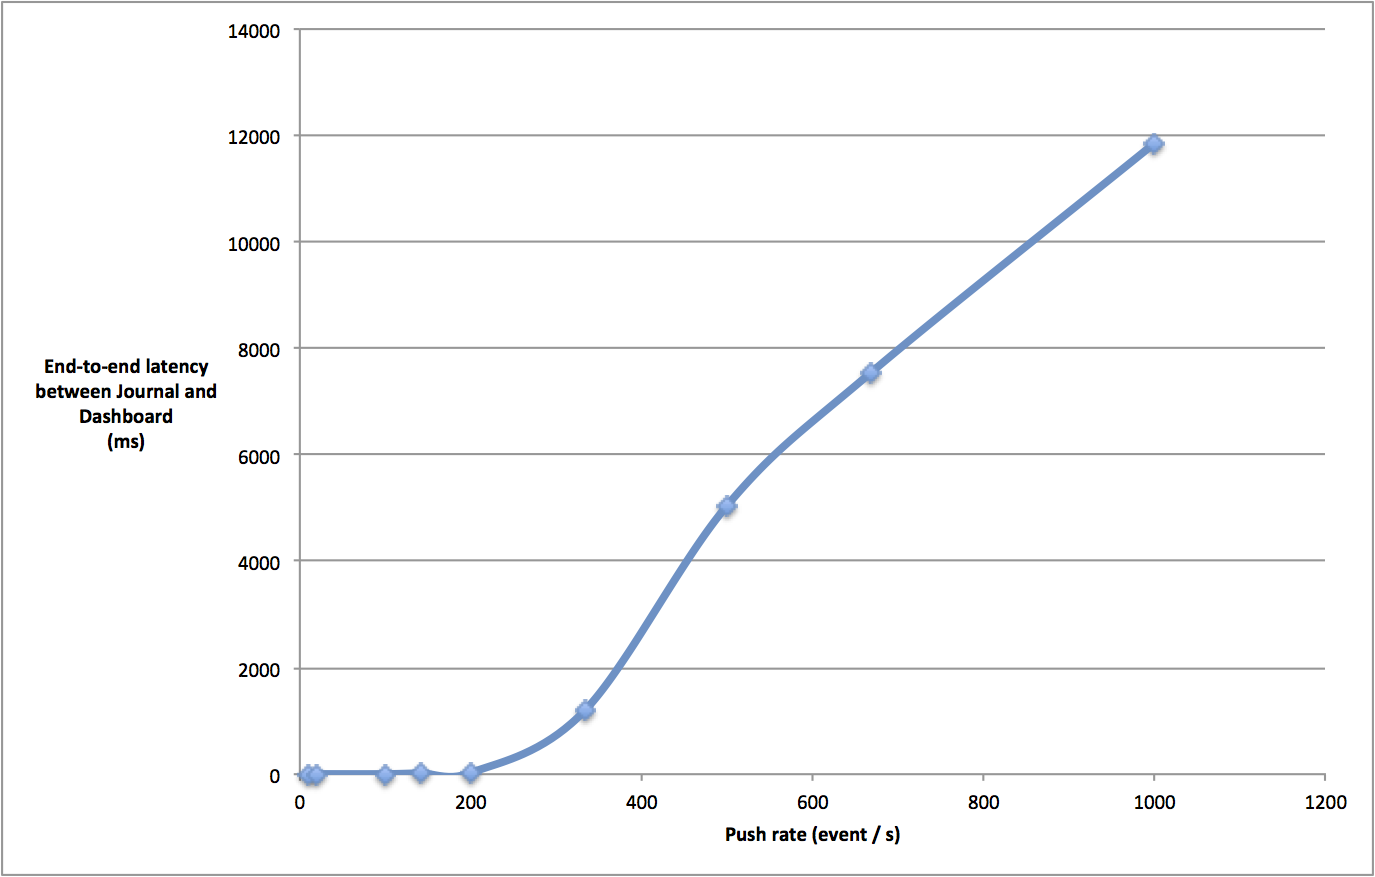
\includegraphics[width=1.0\textwidth]{img/plotlatency.png}}
    \caption{Average latency between the Journal and a Dashboard while varying the Journal push rate}
    \label{fig:latencyplot}
  \end{center}
\end{figure}

Another interesting way to look at these results is to compute the consumption rate of a dashboard, i.e. the inverse of the end-to-end latency. Figure \ref{fig:consumptionrate} shows the plot computed with the data of Figure \ref{fig:latencyplot} by inversing the latency. We see that when the dashboards are up-to-date with the real-time stream (push rate from 0 to 200), the maximum consumption rate is 250 events per second. However, this value decreases rapidly with a push rate higher than 200 events per second, which means that dashboards are late in the stream and don't manage to reduce their lateness.
\\

\begin{figure}
  \begin{center} 
    \makebox[\textwidth]{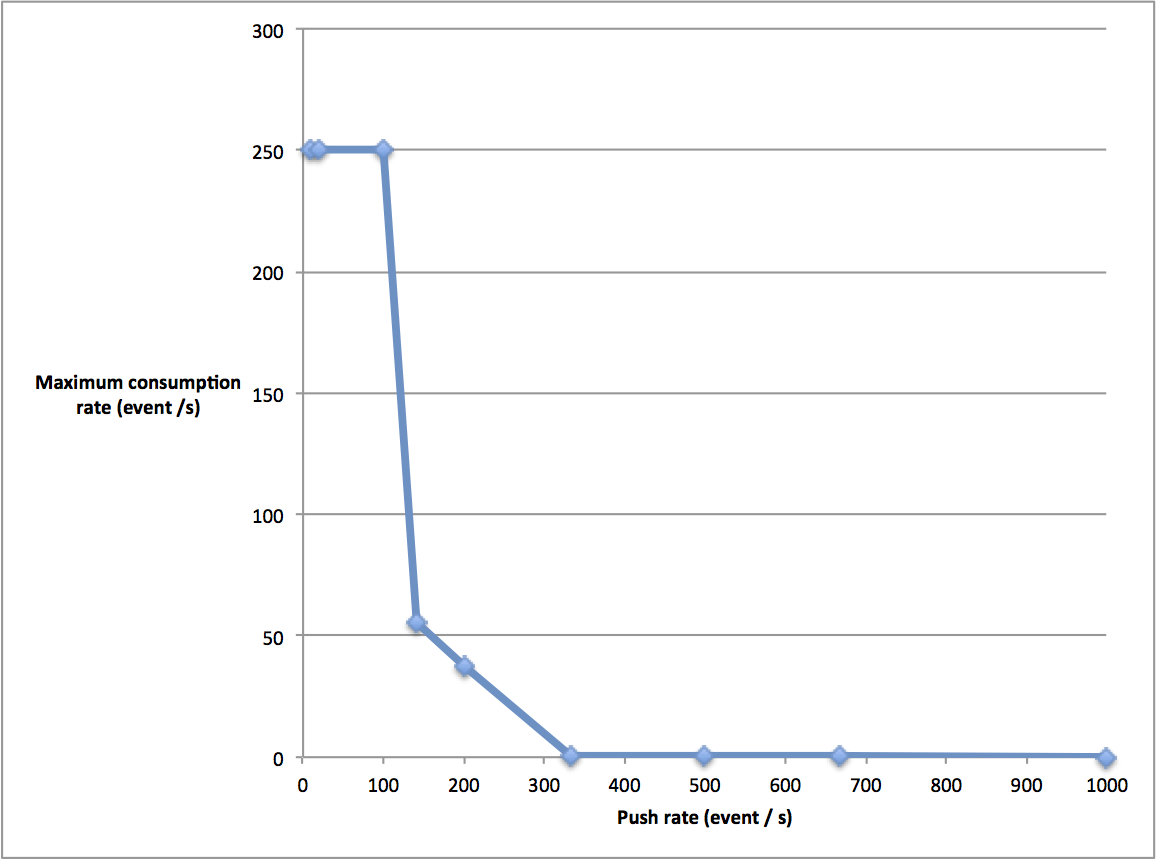
\includegraphics[width=1.0\textwidth]{img/consumptionrate.png}}
    \caption{Maximum consumption rate of a dashboard while varying the Journal push rate}
    \label{fig:latencyplot}
  \end{center}
\end{figure}


To better visualize the fact that low-level processors in the tree (dashboards) can catch up (or not) with the real-time stream speed, Figure \ref{fig:pushrate100}, Figure \ref{fig:pushrate500} and Figure \ref{fig:pushrate1000} show the latency of each event in sequential order for several push rates. 

We see that in Figure \ref{fig:pushrate100} (100 events / s), almost all events have a latency of 4 ms from the beginning of the test. The peaks of latency that happen sometimes are due to garbage collection. However we notice a higher and slightly larger peak at the beginning of the plot (corresponding to the first events). This is due to the initial warm-up of the JVM and the processors.

On Figure \ref{fig:pushrate500} (500 events / s), we see an initial large latency peak, and then the latency goes back to the normal 4 ms with a few latency peaks due to garbage collection. We notice that the initial latency peak is now larger than in the 100 events / s case. This is because the system needs more time to warm-up for a stream at 500 events / s rather than 100 events / s, but then the dashboards manage to catch up with the real-time stream (as their processing speed is still lower than the push rate), and the latency goes back to normal (4 ms) after this warm-up time.

However, in Figure \ref{fig:pushrate1000} (1000 events / s), we notice that the latency goes on increasing. This is because dashboards do not manage to catch up with the real-time stream that is too fast compared to their processing speed, so they keep accumulating lateness compared to the real-time stream. One solution could be to distribute the dashboards on several machines to allow more resource to them. Moreover, in a real-world scenario, one can hope that moments with 1000 events / s are interleaved with moments where the push rate is slower so that the processors have time to reduce their lateness and eventually catch up with the real-time stream. This scenario is simulated in Figure \ref{fig:severalrates}: event 0 to 10000 are pushed with a push rate of 1000 events / s, and just after event 10000 to 20000 are pushed with a push rate of 100 events / s. We see that the processors manage to catch up with the real-time stream around event 12500 and then the latency remains constant at 4 ms.
\\

\begin{figure}
  \begin{center} 
    \makebox[\textwidth]{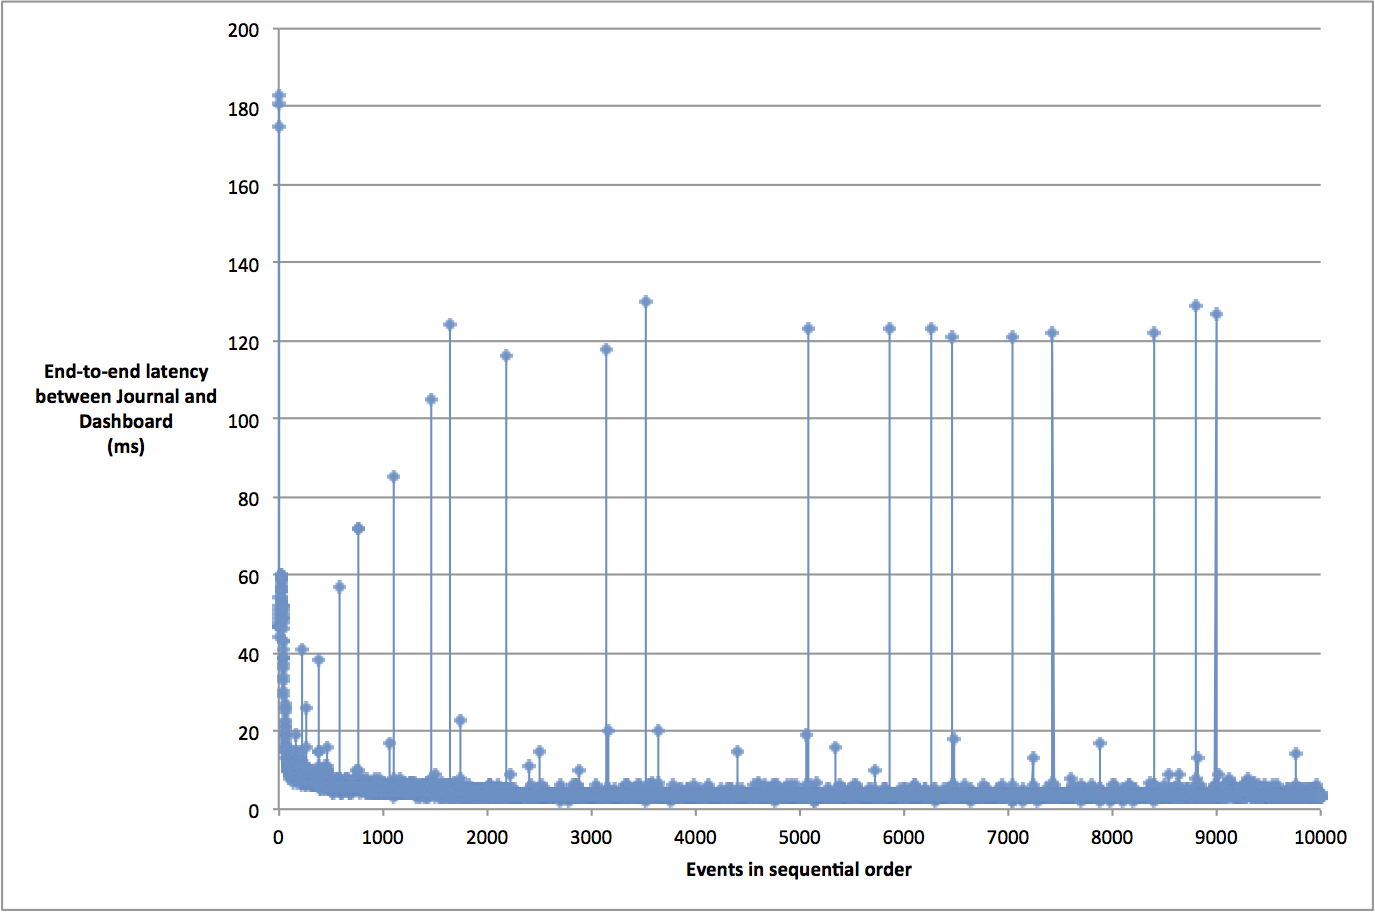
\includegraphics[width=1.0\textwidth]{img/pushrate100.png}}
    \caption{Latency of events between the Journal and a Dashboard with a push rate of 100 events per second}
    \label{fig:pushrate100}
  \end{center}
\end{figure}

\begin{figure}
  \begin{center} 
    \makebox[\textwidth]{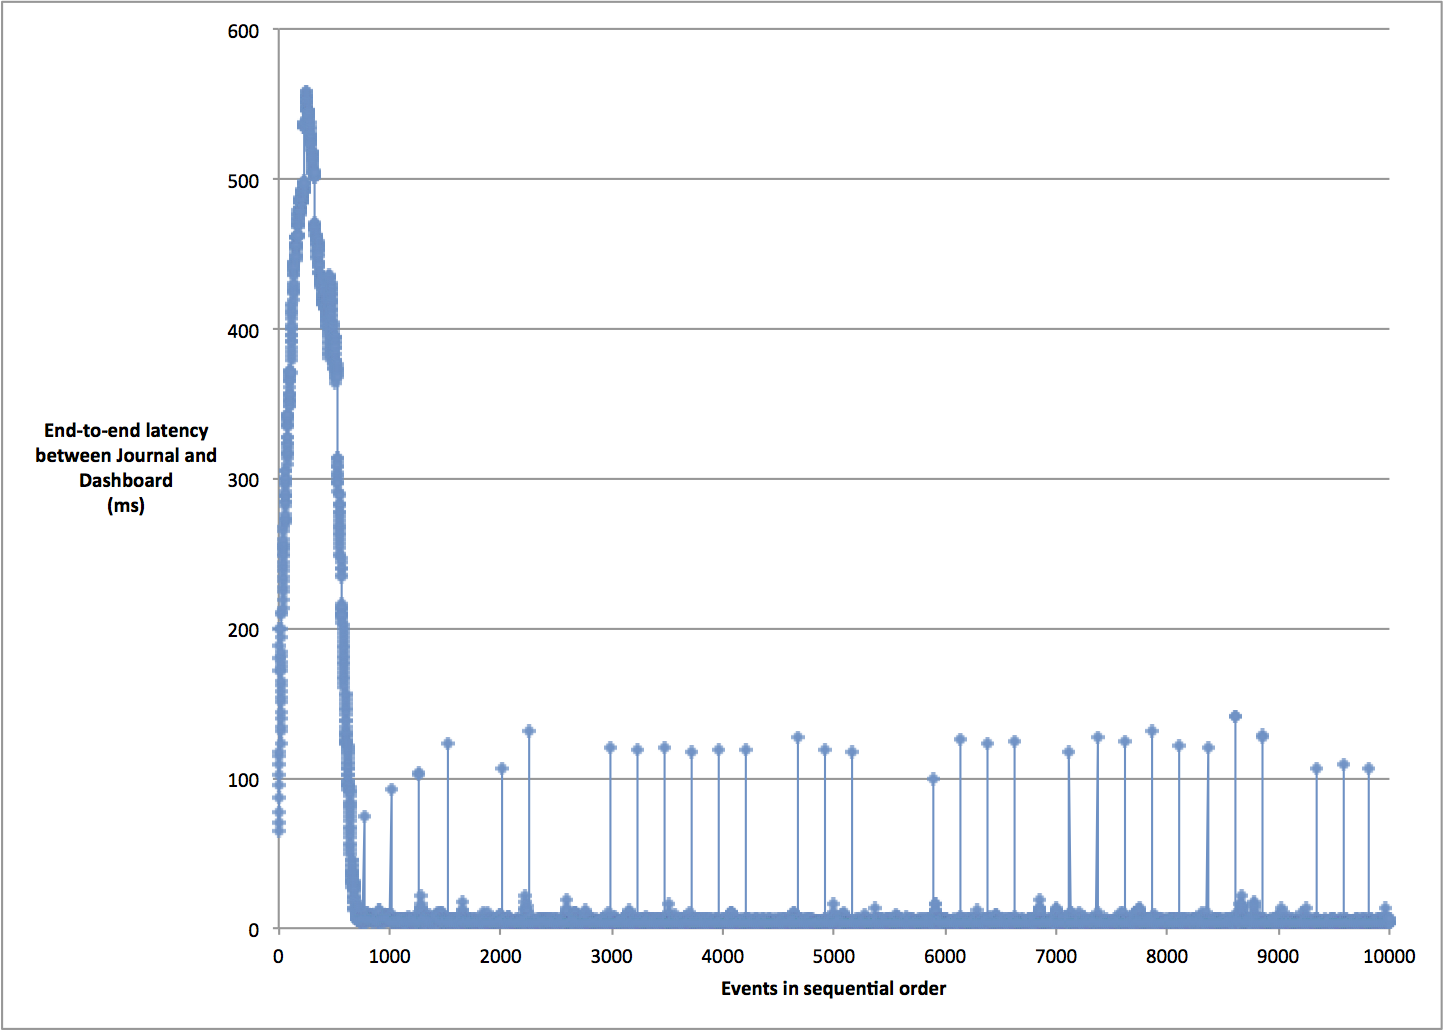
\includegraphics[width=1.0\textwidth]{img/pushrate500.png}}
    \caption{Latency of events between the Journal and a Dashboard with a push rate of 500 events per second}
    \label{fig:pushrate500}
  \end{center}
\end{figure}

\begin{figure}
  \begin{center} 
    \makebox[\textwidth]{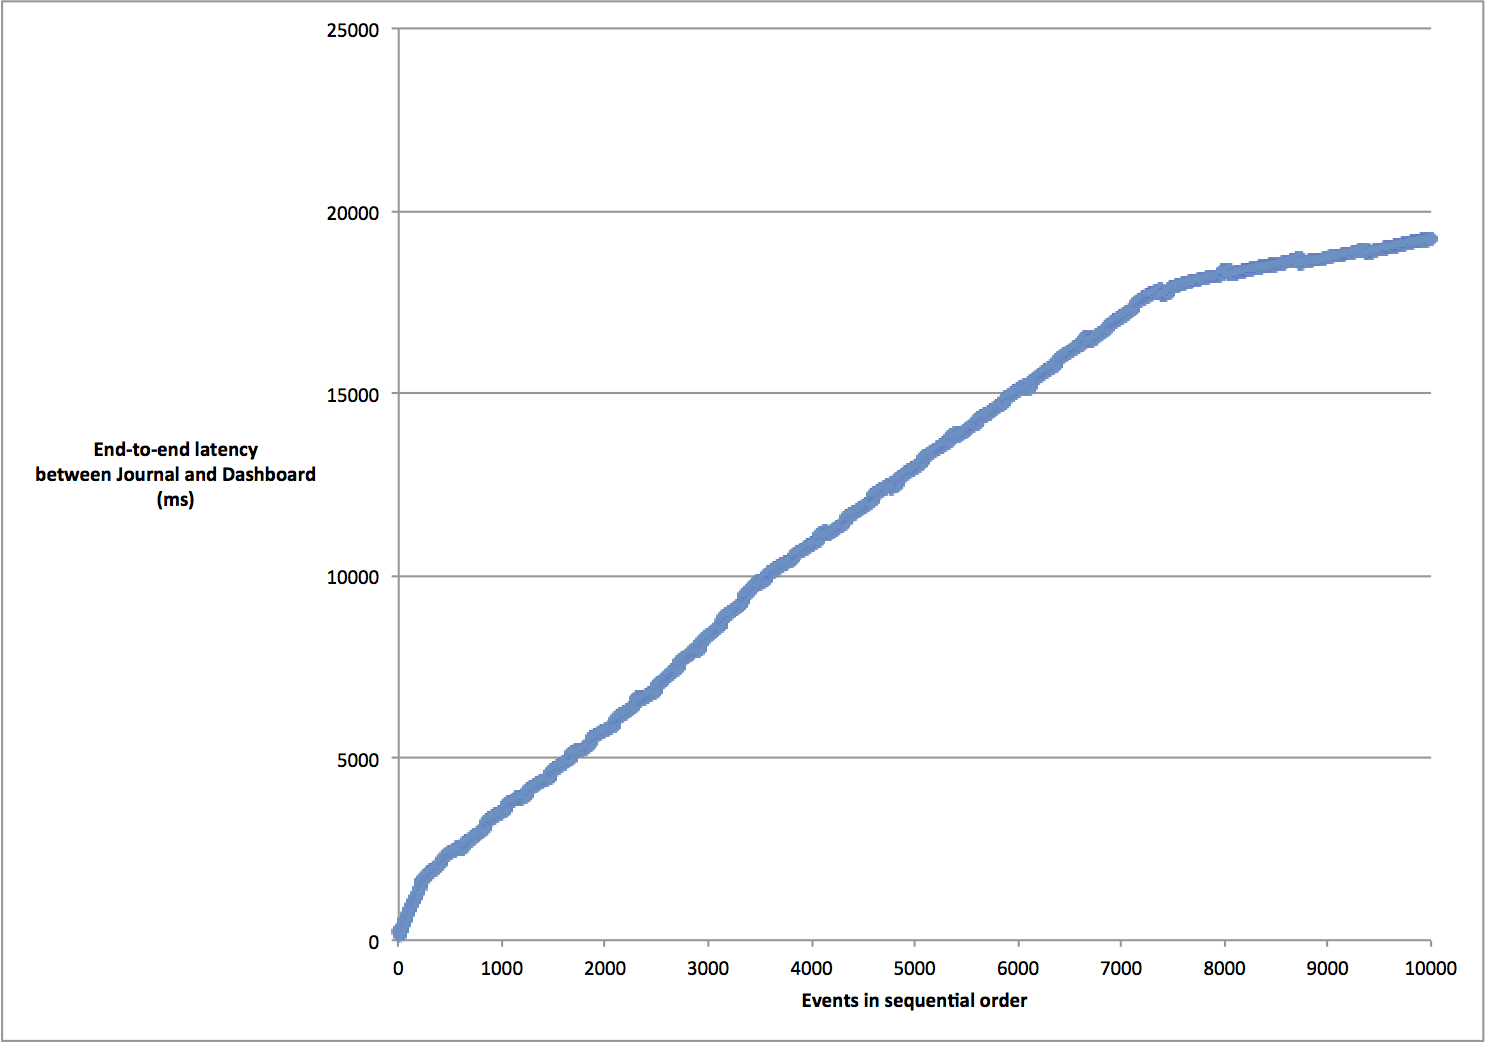
\includegraphics[width=1.0\textwidth]{img/pushrate1000.png}}
    \caption{Latency of events between the Journal and a Dashboard with a push rate of 1000 events per second}
    \label{fig:pushrate1000}
  \end{center}
\end{figure}

\begin{figure}
  \begin{center} 
    \makebox[\textwidth]{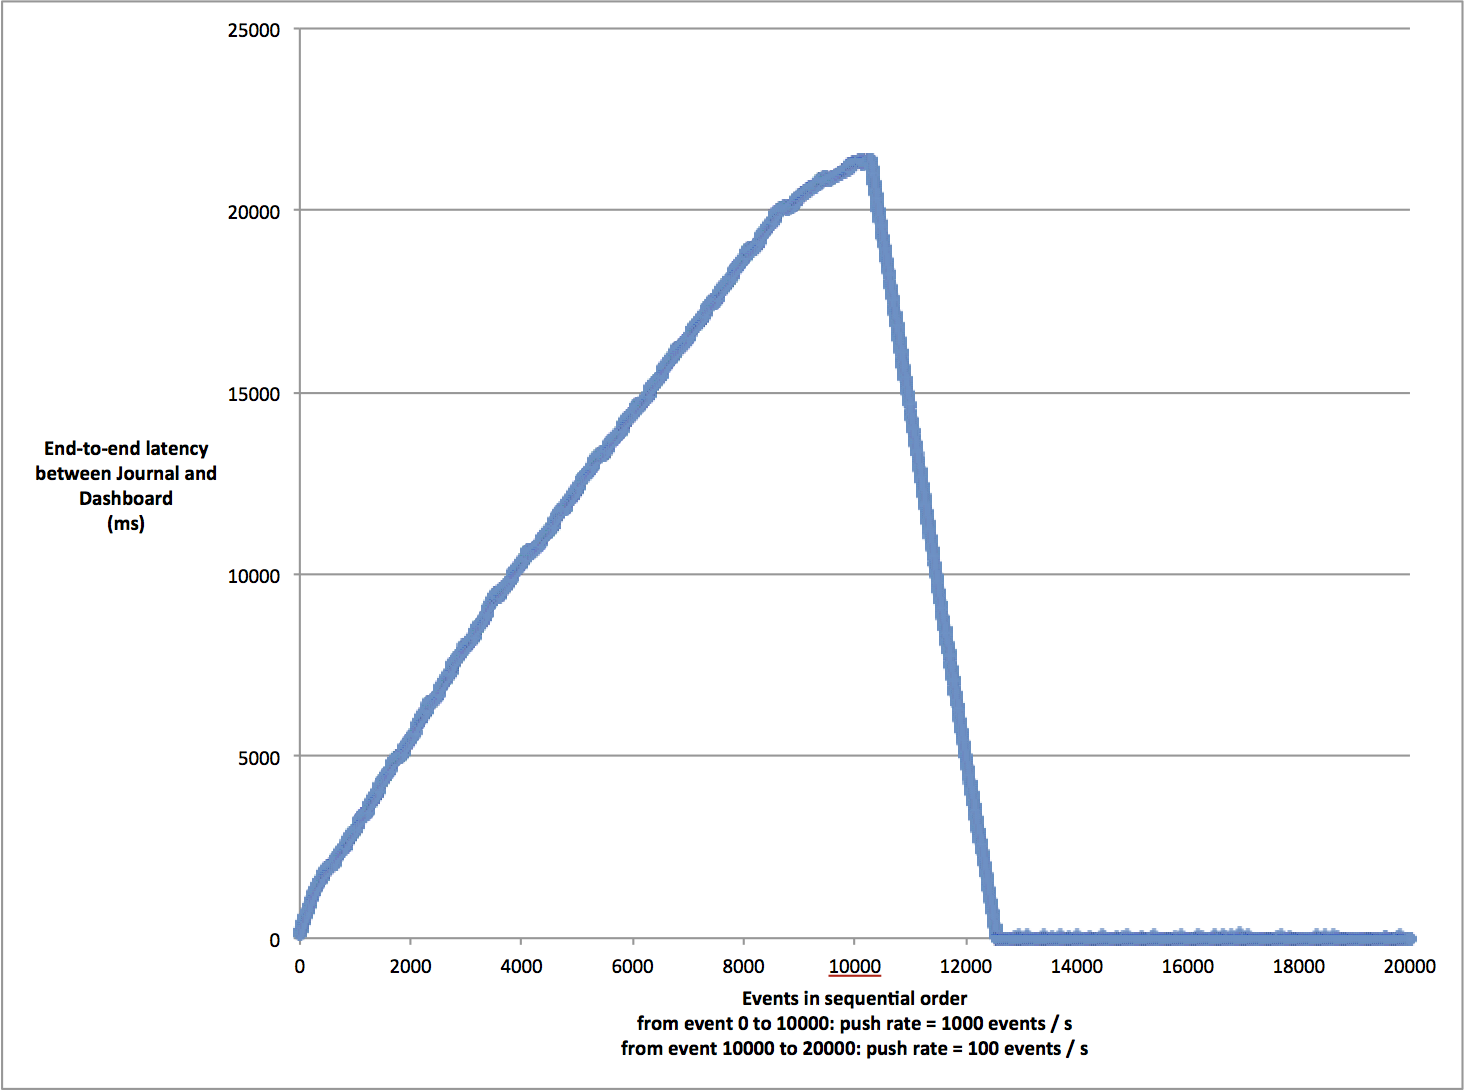
\includegraphics[width=1.0\textwidth]{img/severalrates.png}}
    \caption{Latency of events between the Journal and a Dashboard with variable push rates}
    \label{fig:severalrates}
  \end{center}
\end{figure}

Furthermore, during these performance tests, the resource consumption (JVM Heap space, number of threads) has been profiled. Figure \ref{fig:plotheapspace} and Figure \ref{fig:plotthreads} show the JVM Heap space used and the number of threads used while increasing the event push rate.
Concerning the number of threads used, we notice that this number is constant (76) independently of the push rate, which is expected with our non-blocking IO model to avoid too many thread creations and context switching.
Concerning the JVM heap space consumption, we notice that the value increases in a less than linear fashion with the push rate (the plot has a logarithmic shape).
These two plots validate the fact that the platform uses an amount of resources that does not increase too much with the load (optimization of resource consumption).

\begin{figure}
  \begin{center} 
    \makebox[\textwidth]{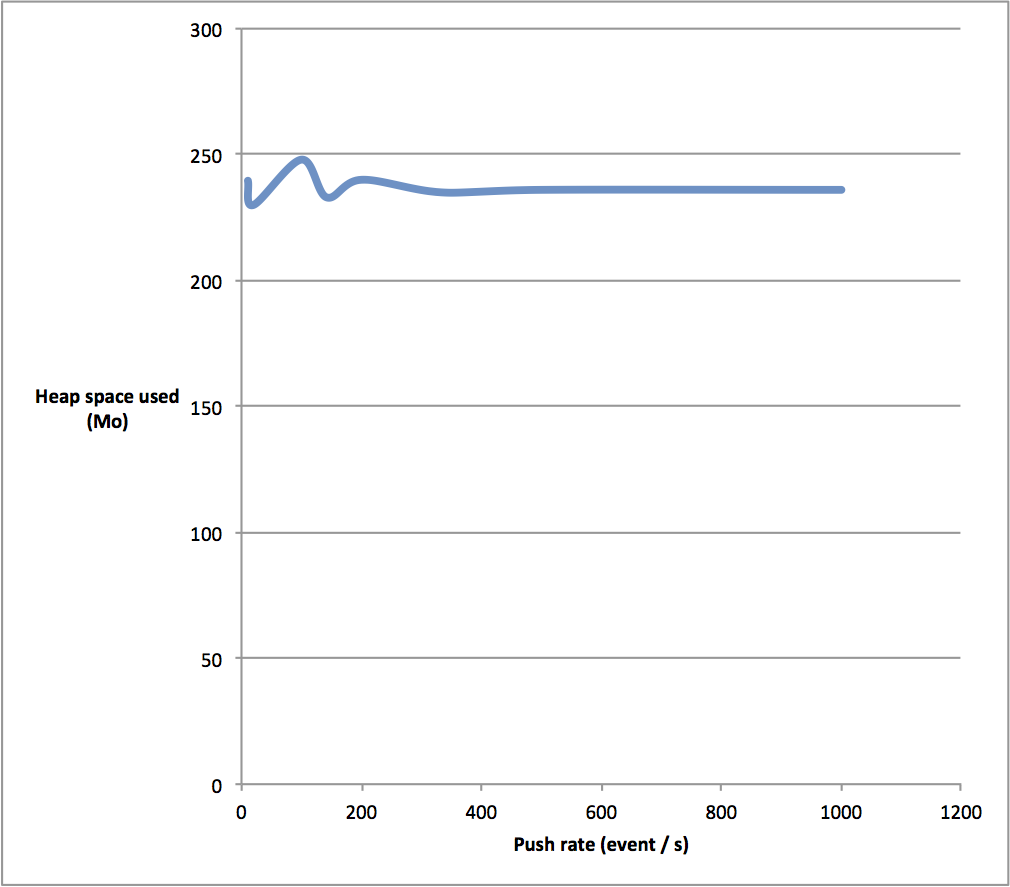
\includegraphics[width=0.8\textwidth]{img/plotheapspace.png}}
    \caption{JVM heap space consumption while varying the Journal push rate}
    \label{fig:plotheapspace}
  \end{center}
\end{figure}

\begin{figure}
  \begin{center} 
    \makebox[\textwidth]{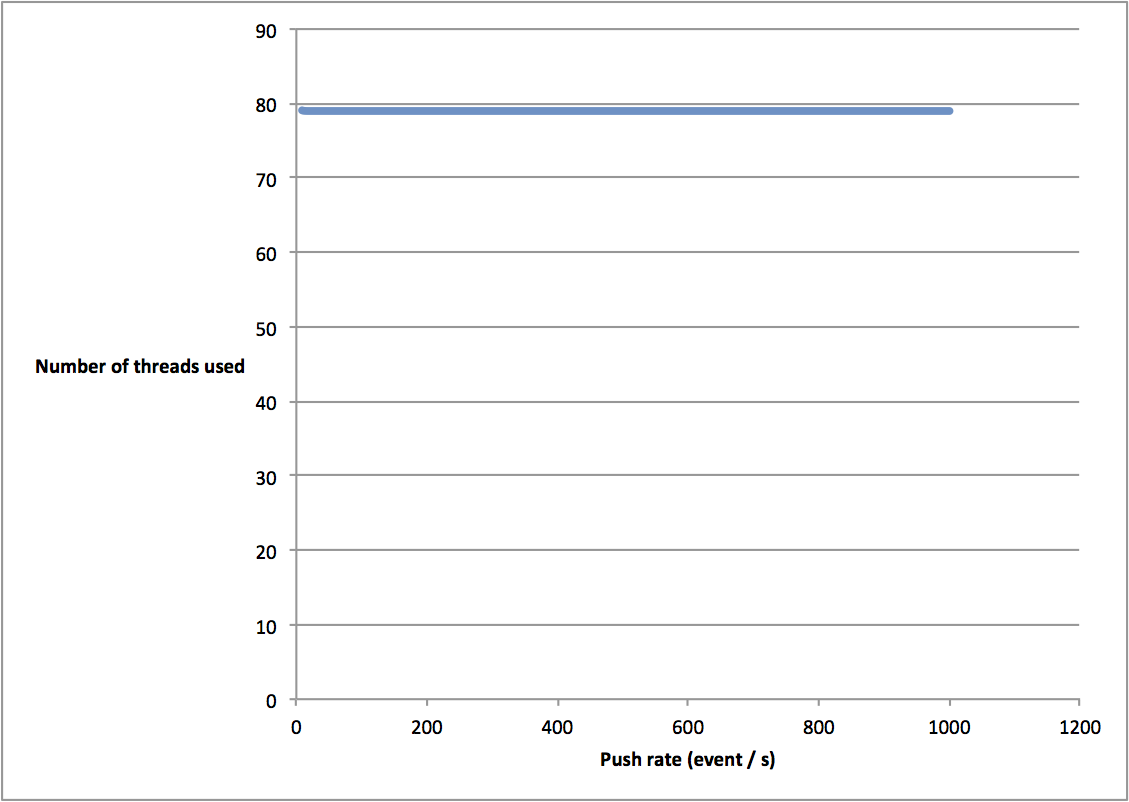
\includegraphics[width=0.8\textwidth]{img/plotthreads.png}}
    \caption{Number of threads used while varying the Journal push rate}
    \label{fig:plotthreads}
  \end{center}
\end{figure}


\section{Fault-tolerance}

In this part, we define a performance test to measure the recovery time of a processor that recovers from a crash and must replay 1000 events that happened when it was crashed. Figure \ref{fig:barchart} shows the resulting bar chart.
Using the tree structure of the business use case application presented in section \ref{sec:usecasebusiness}, the Snapshot processor is first killed and then restarted. Its parent is the Journal, a persistent processor, so it has only one level to climb in the tree to replay the stream. Then, FlatSnapshot is killed. It is at level 2 in the tree, but its parent is a persistent processor (Snapshot), so it has also only one level in the tree to climb to replay the stream. As a result, its replay time is roughly the same than Snapshot (the processing time of these two processors is equivalent). Last but not least, a Dashboard is killed. As its parent is a side-effect processor (FlatSnapshot), it has to climb 2 levels to replay the stream (until reaching the Snapshot persistent processor). Moreover, the processing time of a dashboard is slightly superior than other processors. As a result of these two factors (side-effect parent and slightly longer processing time), we see that Dashboard takes more time to replay the 1000 events that it missed, which is expected according to our model.
\\
\begin{figure}[h]
  \begin{center} 
    \makebox[\textwidth]{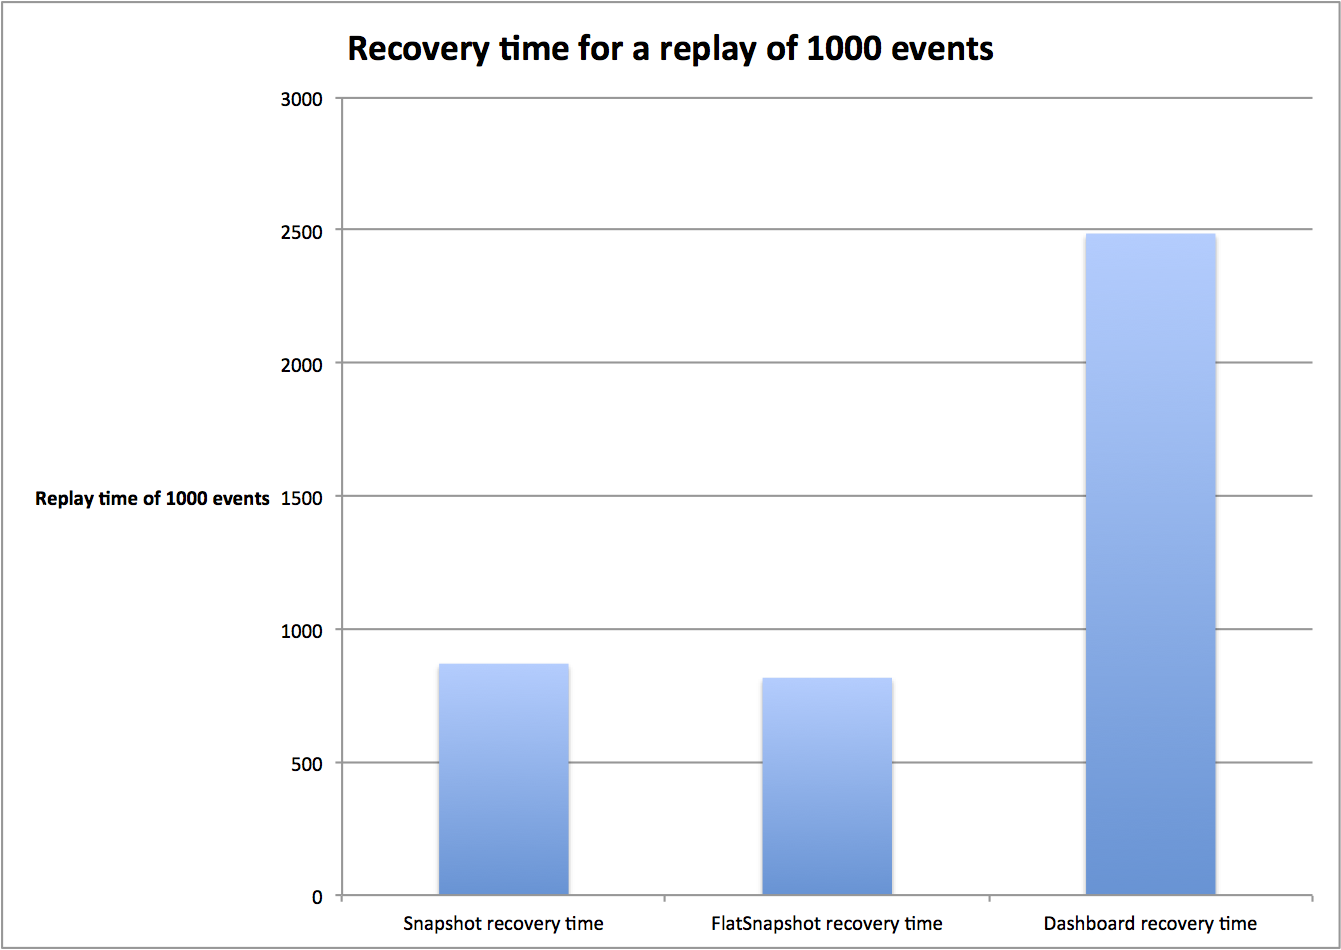
\includegraphics[width=1.0\textwidth]{img/barchart.png}}
    \caption{Recovery time of processors for a replay of 1000 events}
    \label{fig:barchart}
  \end{center}
\end{figure}


\section{Conclusion}

To conclude, the performance tests meet the goals with expected latency patterns (the end-to-end event latency is constant before a push rate threshold from where the dashboards are forced to be late in the stream, but they can reduce their lateness if the push rate decreases after a period of high push rate). Moreover, resource consumption does not increase to much with the push rate. Last but not least, for a push rate of 100 events per seconds (which corresponds to the common push rate for the business application), the end-to-end latency is constant at 4 ms on a local machine, which is a very good result for our use case.






